\Chapter{Introduction}
	\section{Fondamentaux de la physique des plasmas}
		 
		\emph{Le plasma}. Le plasma est souvent considéré un peu équivoquement
		comme le quatrième état de la matière. Dans notre environnement proche,
		nous avons pris conscience de son existence à travers les phénomènes de flammes,
		d'éclairs, d'aurore boréales ou d'arc électriques. Mais à des conditions de
		pressions et de températures différentes de celles de notre atmosphère
		terrestre, il est omniprésent : plus de 99\% de la matière connue est sous
		cette forme. 
		
		En fait le plasma est un gaz conducteur. Une partie des
		particules gazeuses y est ionisée, formant une population
		d'électrons libres et d'ions. Ces populations permettent le transport de
		courant et sont sensibles aux forces électromagnétiques, influençant
		fortement le comportement global du plasma et provoquant des phénomènes
		collectifs, non-linéaires et turbulents.
		
		Le plasma et son comportement sont décrits par la théorie de la physique des
		plasmas. Elle intègre les connaissances de nombreux domaines, tels que la
		physique statitique, l'électromagnétisme, ou encore la dynamique des fluides.
		
		\subsection{Les paramètres plasmas}
		
			Les plasmas se définissent donc comme des gaz possédant une population
			d'électrons libres $n_e$ à une température électronique $T_e$. 
			La figure \ref{zoologie} issue de \cite{national1995Plasma}
			représente une classification des plasmas en fonction de ces deux paramètres 
			principaux qui vont influer sur la dynamique du transport du courant.
			La théorie présentée dans la suite de cette thèse ne concerne que les plasmas
			dits classiques :
			\begin{itemize}
			  \item les plasmas naturels peu dense tels que l'espace interstellaire,
			  le vent solaire, la magnétosphère, et l'ionosphère
			  \item les plasmas naturels denses tels que les éclairs et les étoiles
			  \item les plasmas industriels, de laboratoire, et thermonucléaires
			\end{itemize}
			Dans ces plasmas, le courant se propage de fale transport de la matière suit
			les lois de la mécanique classique et la dynamique du courant \begin{figure}[h]
				\centering
				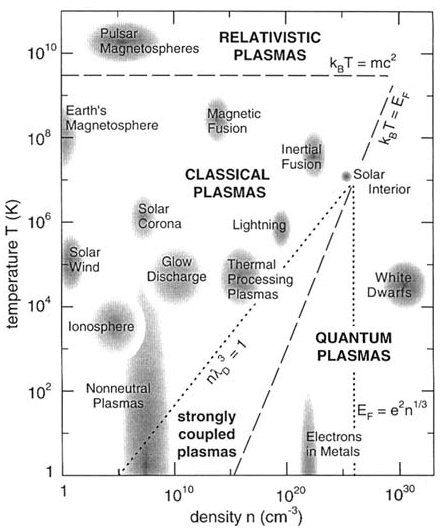
\includegraphics[height=100mm,width=80mm]{figures/zoologie.png}{\caption{Classification
				de différents plasmas en fonction de $n_e$ et $T_e$.}\label{zoologie}}
			\end{figure}
			
			
			
			Le dégré d'ionisation va fortement influencer la nature du transport des courants dans le plasma.
			le paramètre des charges et 
			  
			ont une vitesse supérieure à $c$ la vitesse de la lumière, les effets
			relativistes sont importants. A forte densité, 
			
		
		
		\begin{itemize}
				\item la densité électronique $n_e$ détermine le degré d'ionisation du plasma :
				$$\alpha=\frac{n_e}{n_e+n_i}$$ 
				\item la température électronique $T_e$ définit
			l'agitation thermique et contrôle la cinétique du plasma à travers le paramètre plasma\footnote{Le paramètre 
			plasma représente le ratio
			entre l'énergie thermique des électrons et leur énergie potentielle electrostatique coulombienne 
			\emph{ie.} l'inertie des électrons (et principalement leur agitation thermique desordonnée) contre les forces
			d'interactions coulombiennes structurantes. La tendance au chaos, ou à l'ordonnancement.}
			$$\Gamma=\frac{<E_p>}{<E_c>}=\frac{e^2n_e^{1/3}}{\epsilon_0 kT_e}$$
			\end{itemize}
			
		 Plasma parameter $\Lambda$ Debye sphere, Quasineutrality Debye length,
		Electrostatic plasma frequency $\omega_c$
		 Density : Degree of ionisation $\alpha=n_i/(n_i+n_n)$
			Temperature : Saha equation, thermal equilibrium, Maxwellian energy dist function
			Potentials : Debye sheath, Boltzmann relation
			Magnetization : Hall parameter, Larmor radius, plasma frequency
			\lipsum{50}
		\subsection{Collective behaviour}
			Ambipolar field, heating, drifts
		\subsection{Collisions}
			\lipsum{50}
		\subsection{Scales}
			\lipsum{50}
		
	\section{Fluid description of a plasma}
	\lipsum{50}
		\subsection{Statistical description}
			\subsubsection{BBGKY hierarchy, liouville equation}
			\subsubsection{The Boltzmann equation}
			\lipsum{50}
		\subsection{Moments of the Boltzmann equation, conservation laws}
			Braginskii equations
			\subsubsection{Continuity equation}
			\lipsum{50}
			\subsubsection{Momentum equation}
			\lipsum{50}
			\subsubsection{Energy equation}
			\lipsum{50}
			\subsubsection{Heat equation}
			\lipsum{50}
	\section{Low-temperature plasmas}
		\subsection{Creation of the discharge, role of electrons}
		Dans les plasmas basse-température industriels et de laboratoires, qui possédent
			un faible degré d'ionisation, ou dans l'ionospère, la dynamique du plasma est dominée par
			la perte de quantité de mouvement dûe à l'ionisation la force de friction avec le gaz.
		Electrical breakdown, Townsend avalanche, 
		\lipsum{50}
		\subsection{Ions transport and ambipolar field}
	\section{Edge plasma physics of tokamaks}
		Lawson criteriom, strongly magnetized
		\subsection{Fusion and tokamaks}
		\subsection{Drift velocities}
		\subsection{Turbulence and anomalous transverse transport}
		\lipsum{50}
	\section{Plasma surface interaction and sheath physics}
		\lipsum{50}
		\subsection{Debye sheath}
			\lipsum{50}
		\subsection{Bohm criterium}
			\lipsum{50}
		\subsection{Open field line physics}
			\lipsum{50}
		\subsection{Issue of sheath parallel to the magnetic field}
			\lipsum{50}

		